\documentclass[10pt,a4paper]{article}
\usepackage[utf8]{inputenc}

% \usepackage{ngerman}  % german documents
\usepackage{graphicx}  % import graphics einbinden
\usepackage{listings}  % support source code listing
\usepackage{amsmath}  % math stuff
\usepackage{amssymb} % 
\usepackage{a4wide} % wide pages
\usepackage{fancyhdr} % nice headers
\usepackage{float}
\usepackage{longtable}
\usepackage{xcolor}
\definecolor{darkpastelgreen}{rgb}{0.01, 0.75, 0.24}
\definecolor{spirodiscoball}{rgb}{0.06, 0.75, 0.99}
\definecolor{smalt}{rgb}{0.0, 0.2, 0.6}
\definecolor{armygreen}{rgb}{0.29, 0.33, 0.13}
\definecolor{awesome}{rgb}{1.0, 0.13, 0.32}
\definecolor{bittersweet}{rgb}{1.0, 0.44, 0.37}
\definecolor{bananayellow}{rgb}{1.0, 0.88, 0.21}
\definecolor{blue}{rgb}{0.0, 0.0, 1.0}
\definecolor{red}{rgb}{1.0, 0.0, 0.0}
\definecolor{green}{rgb}{0.0, 1.0, 0.0}



\lstset{basicstyle=\footnotesize,language=Python,breaklines=true,numbers=left, numberstyle=\tiny, stepnumber=5,firstnumber=0, numbersep=5pt} % set up listings
\pagestyle{fancy}             % header
\setlength{\parindent}{0pt}   % no indentation

\usepackage[pdfpagemode=None, colorlinks=true,  % url coloring
           linkcolor=blue, urlcolor=blue, citecolor=blue, plainpages=false, 
           pdfpagelabels,unicode]{hyperref}
           
% change enums style: first level (a), (b), (c)           
\renewcommand{\labelenumi}{(\alph{enumi})}
\renewcommand{\labelenumii}{(\arabic{enumii})}

\newcommand{\norm}[1]{\left\lVert#1\right\rVert}

%lecture name
\newcommand{\lecture}{
	Bioinformatics III
}           

%assignment iteration
\newcommand{\assignment}{
	Fourth Assignment
}


%set up names, matricle number, and email
\newcommand{\authors}{
  \begin{tabular}{rl}
    \href{mailto:s8tbscho@stud.uni-saarland.de}{Thibault Schowing} & (2571837)\\
    \href{mailto:wiebkeschmitt@outlook.de}{Wiebke Schmitt} & (2543675)
  \end{tabular}
}

% use to start a new exercise
\newcommand{\exercise}[1]
{
  \stepcounter{subsection}
  \subsection*{Exercise \thesubsection: #1}

}

\begin{document}
\title{\Large \lecture \\ \textbf{\normalsize \assignment}}
\author{\authors}

\setlength \headheight{25pt}
\fancyhead[R]{\begin{tabular}{r}\lecture \\ \assignment \end{tabular}}
\fancyhead[L]{\authors}


\setcounter{section}{4} % modify for later sheets, i.e. 2, 3, ...
%\section{Introduction to Python and some Network Properties} % optional, note that section invocation sets the section counter + 1, so adapt the setcounter command
\maketitle

%WIEBKE !!! READ THIS !!! 
% Usefull with Latex and maths: a list of the symbols ! https://reu.dimacs.rutgers.edu/Symbols.pdf

%EXERCICE 1
\exercise{ Dijkstra’s algorithm for finding shortest paths }
\begin{enumerate}

% A
\item \textit{Draw a directed or undirected graph with at least one negative edge weight for which Dijkstra’s
	algorithm does not find the shortest path from some node s to another node t. Use
	your example to explain why Dijkstra’s algorithm only works on graphs with non–negative
	edge weights.}\\

\begin{figure}[H]
	\centering
	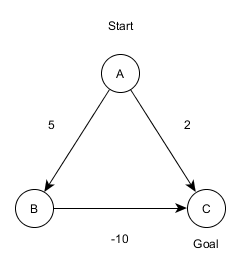
\includegraphics[width=0.5\linewidth]{1a}
	\caption{Example directed graph}
	\label{fig:1a}
\end{figure}

A-B-C is the shortest path. 

We have $ V = {A, B, C} $, $E = {(A,C,2), (A,B,5), (B,C,-10)}$. So, A-C is found first but not A-B-C. 
Dijkstra assume that the minimality will never change when "closing" a node. The use of negative numbers change this rule and so is not compatible with Dijkstra. 


% B
\item \textit{Dijkstra’s algorithm modifications}


\begin{figure}[H]
	\centering
	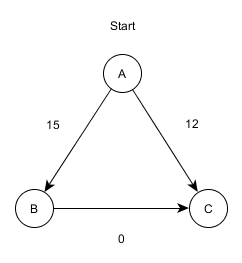
\includegraphics[width=0.5\linewidth]{1b}
	\caption{Graph with edge cost $\geq 0$.}
	\label{fig:1b}
\end{figure}

We can see that adding 10 to all weights doesn't work. A-C is still the path that Dijkstra find first and in this case, it is the shortest path which was not the case before. 




% C
\item \textit{Could BFS be used to find the shortest paths between nodes?
	If so, what would the edge weights have to look like for BFS to be guaranteed to find the
	shortest paths between nodes? Why (not)?}

With BFS, we can find a path with arbitrary weights but it is not guaranteed to be optimal. 

\begin{figure}[H]
	\centering
	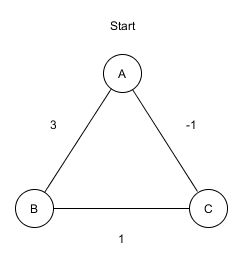
\includegraphics[width=0.5\linewidth]{1c}
	\caption{When we want to go from A to B, the shortest path is A - C - B, but with BFS we will first expand A and find the path A-B. When we expand the C node, B is already marked as "duplicate". BFS will ignore the link between B and C in this case.}  
	\label{fig:1c}
\end{figure}




\end{enumerate}


% NEW EXERCICE
\newpage
\exercise{Force directed layout of networks}
\begin{enumerate}
	
	% A
	\item \textit{Implementation preparation}
	
	For the harmonic force we have: 
	
	
\[ F_{h}(\vec{r}) = -\nabla E_{h}(\vec{r})\]
According to the definition: 
\[ = -\nabla \frac{k}{2} \norm{\vec{r}}^2 = -\frac{k}{2} \nabla \norm{\vec{r}}^2 \]
\[ = -\frac{k}{2}\nabla  (\sqrt{x^2 + y^2 + z^2})^2  \]
\[ = -\frac{k}{2}\nabla  (x^2 + y^2 + z^2)  \]
\[ = -\begin{pmatrix}
kx\\
ky\\
kz
	\end{pmatrix} \]


	For the Coulomb force we have: 
	
	\[ F_{c}(\vec{r}) = -\nabla E_{c}(\vec{r})\]

	\[ = -\nabla(\frac{1}{4\pi\epsilon_{0}} \frac{q1 q2}{\norm{\vec{r}}}) \]
	
	\[ = -\nabla(\frac{1}{4\pi\epsilon_{0}} \frac{q1 q2}{\sqrt{x^2 + y^2 + z^2}}) \]
	
	\[ = - \frac{q1 q2}{4\pi\epsilon_{0}} \nabla ( \frac{1}{\sqrt{x^2 + y^2 + z^2}}) \]
	
	We apply partial derivatives on $ \frac{1}{\sqrt{x^2 + y^2 + z^2}}$ (chain rule): 
	
	\[ = - \frac{q1 q2}{4\pi\epsilon_{0}} \begin{pmatrix}
	-\frac{x}{(x^2 + y^2 + z^2)^{\frac{3}{2}}}\\
	-\frac{y}{(x^2 + y^2 + z^2)^{\frac{3}{2}}}\\
	-\frac{z}{(x^2 + y^2 + z^2)^{\frac{3}{2}}}
	\end{pmatrix} = \frac{q1 q2}{4\pi\epsilon_{0}} \begin{pmatrix}
	\frac{x}{(x^2 + y^2 + z^2)^{\frac{3}{2}}}\\
	\frac{y}{(x^2 + y^2 + z^2)^{\frac{3}{2}}}\\
	\frac{z}{(x^2 + y^2 + z^2)^{\frac{3}{2}}}
	\end{pmatrix} \]
	
	
	
	% B
	\item \textit{\textbf{Adapting the energy equations for networks}}
	
	For the Harmonic force we have: 
	
	%\[ F_{h}(\vec{r}_{i,j}) = -\nabla E_{h}(\vec{r}_{i,j})  \]
	
	%K is the spring constant, because it's constant we can drop it: 
	%\[ F_{h}(\vec{r}_{i,j}) = -\nabla\frac{1}{2} \norm{\vec{r}}^2 \]
	
	%\[-\frac{1}{2} \nabla\left(\sqrt{(x_i - x_j)^2 + (y_i - y_j)^2 }\right)^2 = -\frac{1}{2} \nabla(x_i - x_j)+(y_i - y_j) \]
	
%We apply the partial derivatives: 
	
	%\[= -\frac{1}{2} \begin{pmatrix}
%	y_i - y_j\\
%	x_i - x_j
%	\end{pmatrix} \]


%	OR : 
	
	\[ F_{h}(\vec{r}_{ij}) = -\nabla E_{h}(\vec{r}_{i,j})  = -\begin{pmatrix}
	x_i - y_j\\
	y_i - y_j
	\end{pmatrix} \]

	
	For the Coulomb force:
	
	\[F_{c}(\vec{r_{ij}}) = k_1 k_2 \begin{pmatrix}
	\frac{x_i - x_j}{\left( (x_i - x_j)^2 + (y_i - y_j)^2 \right)^{\frac{3}{2}}}\\
	\frac{y_i - y_j}{\left( (x_i - x_j)^2 + (y_i - y_j)^2 \right)^{\frac{3}{2}}}
	\end{pmatrix} \]

	% C
	\item \textit{\textbf{Understanding the Coulomb and harmonic energy:} How does the Coulomb energy and harmonic energy change if the degree of both nodes is increased or decreased? What happens if the distance between two nodes is increased or decreased?}
	
	%NOT Sure what the "spring constant" is for the harmonic and neither what the harmonic energy is... (something with attraction for connected nodes)
			
		%	Here we will only have degrees $\geq 0$ which means that all the force are going to be repulsive. 
		If the degree of both nodes increases, the harmonic force is not affected but Coulomb force will increase with a factor $ -k_1 k_2 $ as seen in (b). \\
		
		However, if the distance increase, both Coulomb and harmonic will be affected. The Harmonic energy is  $\frac{1}{2}||\vec{r^2}||^2$ and the Coulomb $ \frac{k_i k_j}{||\vec{r}_{ij}||} $ so if we increase the distance, Coulomb energy is going to decrease and Harmonic energy to increase. 
	
	
	% D
	\item \textit{\textbf{\textbf{Understanding the forces:} Why is the Coulomb force the repulsive force and the harmonic force the attractive force?}}
		
		% The harmonic force is here only if there is an edge. Keep connected nodes together and try to repulse the non connected part away. 
		In our case, all the node will have a positive charge (the degree) which means that they are all going to repel each other. However, the objective is to keep connected nodes close to each other and at the same time spread the rest of the graph away to give it a nice display. The Coulomb force is the basic force between every node according to their degrees and distance, disregarding their connection. The Harmonic force is applied here only when two nodes are connected to each other and because it has opposite sign, as seen in (b), it will temper the force between the two connected nodes and allow to keep them close ot each other.  
		
	
	
	% E
	\newpage
	\item \textit{\textbf{Implementing the force directed layout algorithm}}
	
		\lstinputlisting[label=lst-1, caption={layout\string_main.py}] {../Scripts/layout\string_main.py}
		\lstinputlisting[label=lst-1, caption={layout.py}] {../Scripts/layout.py}
		\lstinputlisting[label=lst-1, caption={node.py}] {../Scripts/node.py}
		\lstinputlisting[label=lst-1, caption={tools.py}] {../Scripts/tools.py}
		\lstinputlisting[label=lst-1, caption={generic\string_network.py}] {../Scripts/generic\string_network.py}
		
		
		
		
	
	% F
	\newpage
	\item \textit{\textbf{Simulated annealing:} Explain why simulated annealing is a worthwhile optimisation principle in practice.}\\
	 % first position random -> might have a long distance to do before beeing in the right place -> first big coarse moves to lower the big gapes
	Simulated annealing will approximate the global minimum (unlike Gradient descent, which will find a precise local minima). These methods avoid getting stuck in a local minima by making big random jumps in the beginning and reduce their size as we stabilize the layout. If a node is "stuck" in a force-field in which it does not belong,see figure \ref{fig:dognormalerror}, a random force might help it to get out. If a node is already in a good position, this random force might false a little bit the scheme but won't break the overall structure. As the temperature is decreasing, the random force won't have the ability to displace the node far away of their position. The more iterations, the less amount of temperature. \\
	
	
	
	% G
	\item \textit{\textbf{Applying the layout algorithms}}\\
	
	
\begin{figure}[H]
	\centering
	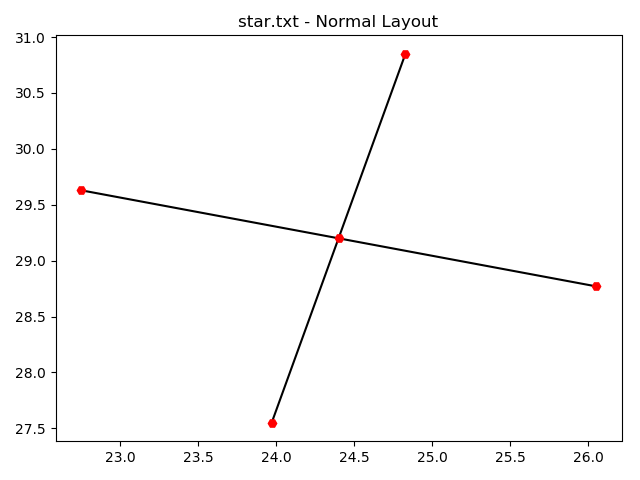
\includegraphics[width=0.5\linewidth]{../Scripts/star_normal}
	\caption{}
	\label{fig:starnormal}
\end{figure}

\begin{figure}[H]
	\centering
	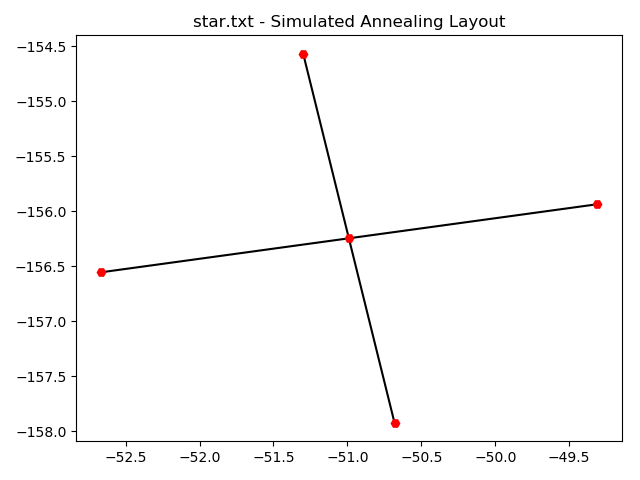
\includegraphics[width=0.5\linewidth]{../Scripts/star_annealing}
	\caption{}
	\label{fig:starannealing}
\end{figure}


\begin{figure}[H]
	\centering
	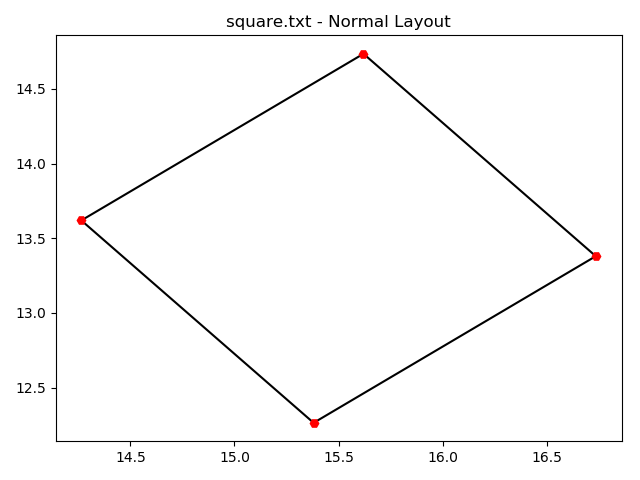
\includegraphics[width=0.5\linewidth]{../Scripts/square_normal}
	\caption{}
	\label{fig:squarenormal}
\end{figure}

\begin{figure}[H]
	\centering
	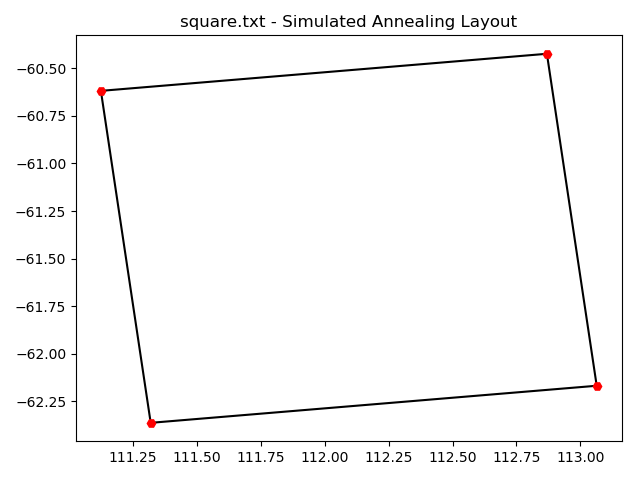
\includegraphics[width=0.5\linewidth]{../Scripts/square_annealing}
	\caption{}
	\label{fig:squareannealing}
\end{figure}

\begin{figure}[H]
	\centering
	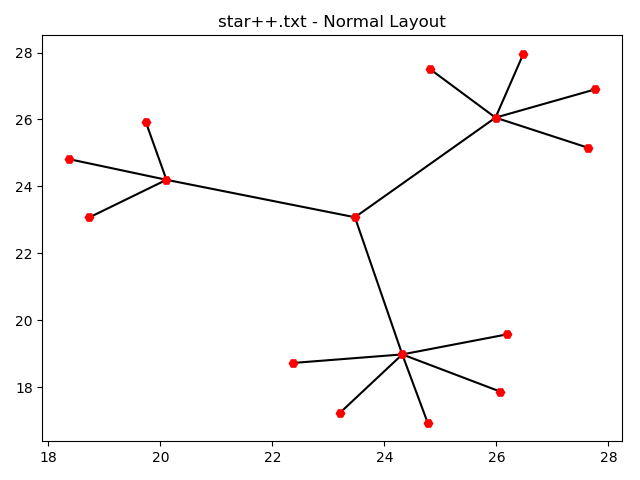
\includegraphics[width=0.5\linewidth]{../Scripts/star++_normal}
	\caption{}
	\label{fig:starpnormal}
\end{figure}

\begin{figure}[H]
	\centering
	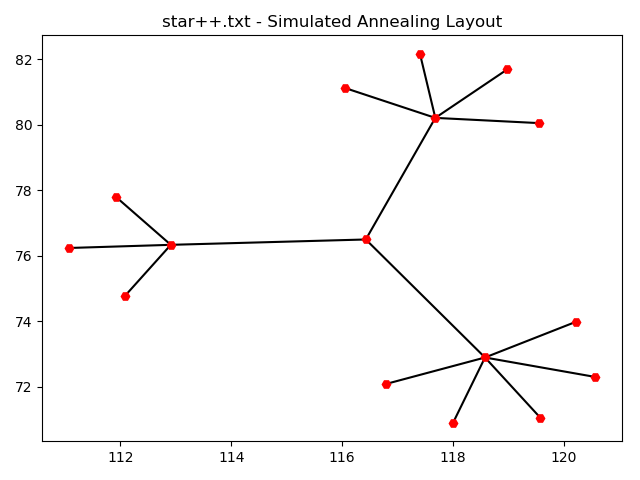
\includegraphics[width=0.5\linewidth]{../Scripts/star++_annealing}
	\caption{}
	\label{fig:starpannealing}
\end{figure}

\begin{figure}[H]
	\centering
	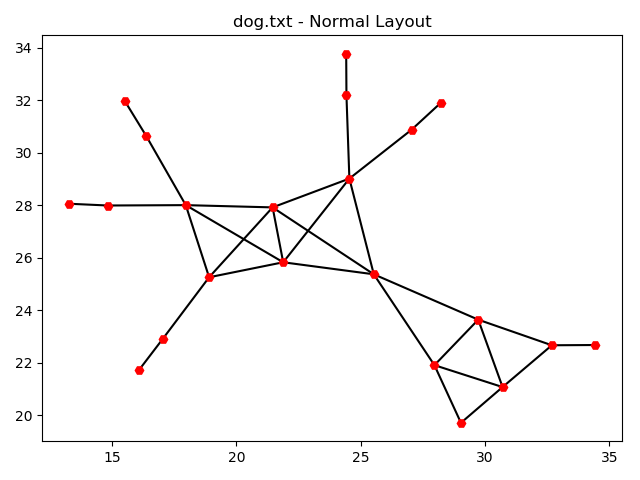
\includegraphics[width=0.5\linewidth]{../Scripts/dog_normal}
	\caption{}
	\label{fig:dgnormal}
\end{figure}

\begin{figure}[H]
	\centering
	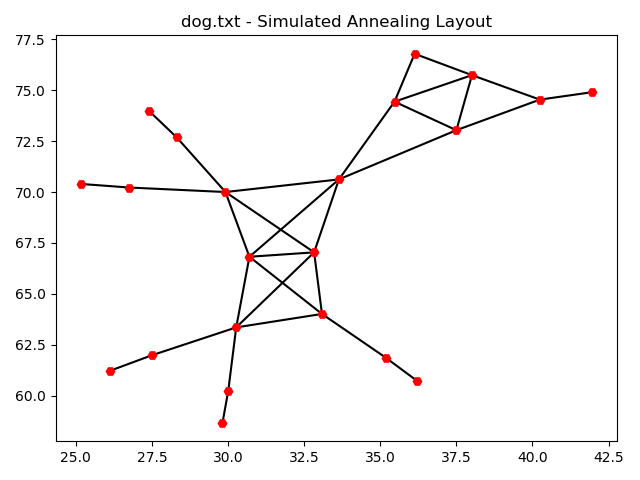
\includegraphics[width=0.5\linewidth]{../Scripts/dog_annealing}
	\caption{}
	\label{fig:dgannealing}
\end{figure}


\begin{figure}[H]
	\centering
	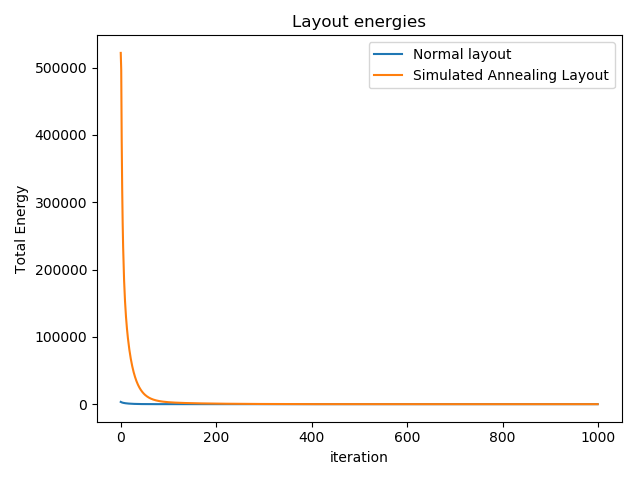
\includegraphics[width=0.7\linewidth]{../Scripts/star++_energies}
	\caption{Energies for the star++ graph}
	\label{fig:starenergies}
\end{figure}

We can see in figure \ref{fig:starenergies}, the total energy lower quicker with the normal layout than with the Simulated Annealing. Both meet around zero after around 200 iterations. 


As said in (f), a node can randomly get stuck somewhere where the forces can't simply make it move and the Simulated Annealing can be useful. In figure \ref{fig:dognormalerror}. After having ran the simulations many times, no such error appeared when using the Simulated Annealing layout. 

\begin{figure}[H]
	\centering
	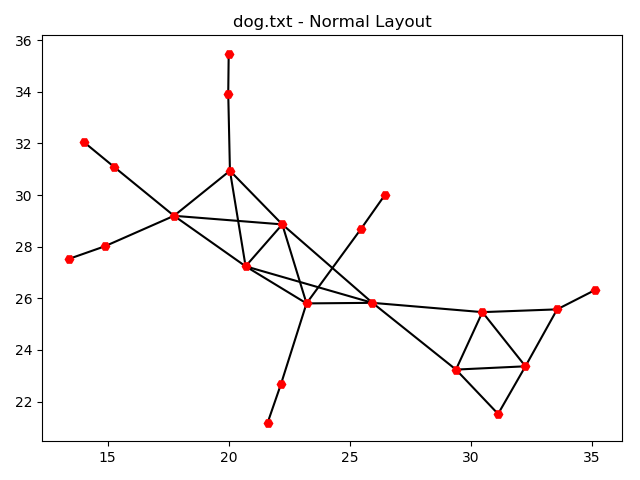
\includegraphics[width=0.7\linewidth]{../Scripts/dog_normal_error}
	\caption{One of the dog's front leg got stuck trying to catch a ball on his back. }
	\label{fig:dognormalerror}
\end{figure}





\end{enumerate}











% NEW EXERCICE
\newpage
\exercise{Graph Modular Decomposition}

\begin{figure}[H]
	\centering
	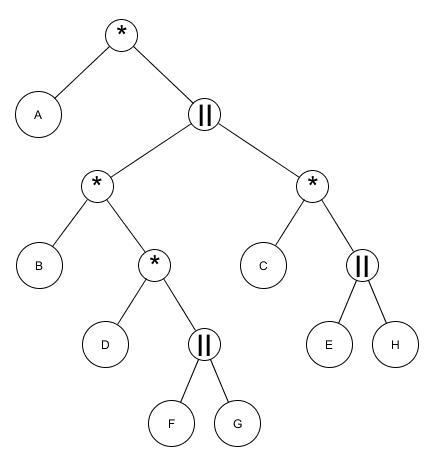
\includegraphics[width=0.7\linewidth]{modulardecomposition}
	\caption{Modular decomposition of the network}
	\label{fig:modulardecomposition}
\end{figure}





\end{document}